\documentclass[11p]{article}
% Packages
\usepackage{amsmath}
\usepackage{graphicx}
\usepackage[swedish]{babel}
\usepackage[
    backend=biber,
    style=authoryear-ibid,
    sorting=ynt
]{biblatex}
\usepackage[utf8]{inputenc}
\usepackage[T1]{fontenc}
%Källor
\addbibresource{mall.bib}
\graphicspath{ {./images/} }

\title{PMmall \\ \small Fysik 1}
\author{Alvin Högdal }
\date{\today}

\begin{document}


    \begin{titlepage}
        \begin{center}
            \vspace*{1cm}

            \Huge
            \textbf{PM energiförsörjning }

            \vspace{0.5cm}
            \LARGE
            Subtitle

            \vspace{1.5cm}

            \textbf{Alvin Högdal}

            \vfill


            Fysik 1

            \vspace{0.8cm}

            
\includegraphics[width=0.4\textwidth]{../images/NTI Gymnasiet_Symbol_print_svart.png}

            \Large
            Teknikprogrammet\\
            NTI Gymnasiet\\
            Umeå\\
            \today

        \end{center}
    \end{titlepage}
% Om arbetet är långt har det en innehållsförteckning, annars kan den utelämnas
    \tableofcontents
    \newpage

    \section{Inledning}
    Vi alla vet vad ett kärnkraftverk är.
    Det är en byggnad som producerar enorma mängder el och radioaktivt avfall.
    Men hur fungerar ett kärnkraftverk, vad händer med det radioaktiva avfallet och vad är konsekvenserna av att gräva efter uranium?
    \subsection{frågeställningar}

    \begin{enumerate}
        \item Hur fungerar ett kärnkraftverk?
        \item Vad händer med det radioaktiva avfallet?
        \item Vad är miljö konsekvenserna av att gräva uranium?
    \end{enumerate}

    \section{Resultat}
    Här kommer allt med massor av mer rubriker och underrubriker
    \subsection{Kärnkraft, så fungerar det}
En kärnreaktor tar kärnbränsle för att starta och kontrolera kärnreaktioner.
Den vanligaste reaktorn tar uranium 235 vilket sönderfaller som fission till barium 141, krypton 92 och 3 neutroner.
Barium och krypton är radiokativt men vi kan inte göra någonting med dom så det blir vad som kallas radioaktivt avfall.
Neutronerna absorberas antingen av kontrollstavar eller annat uranium vilket startar andra fission reaktioner.
    \begin{figure}
        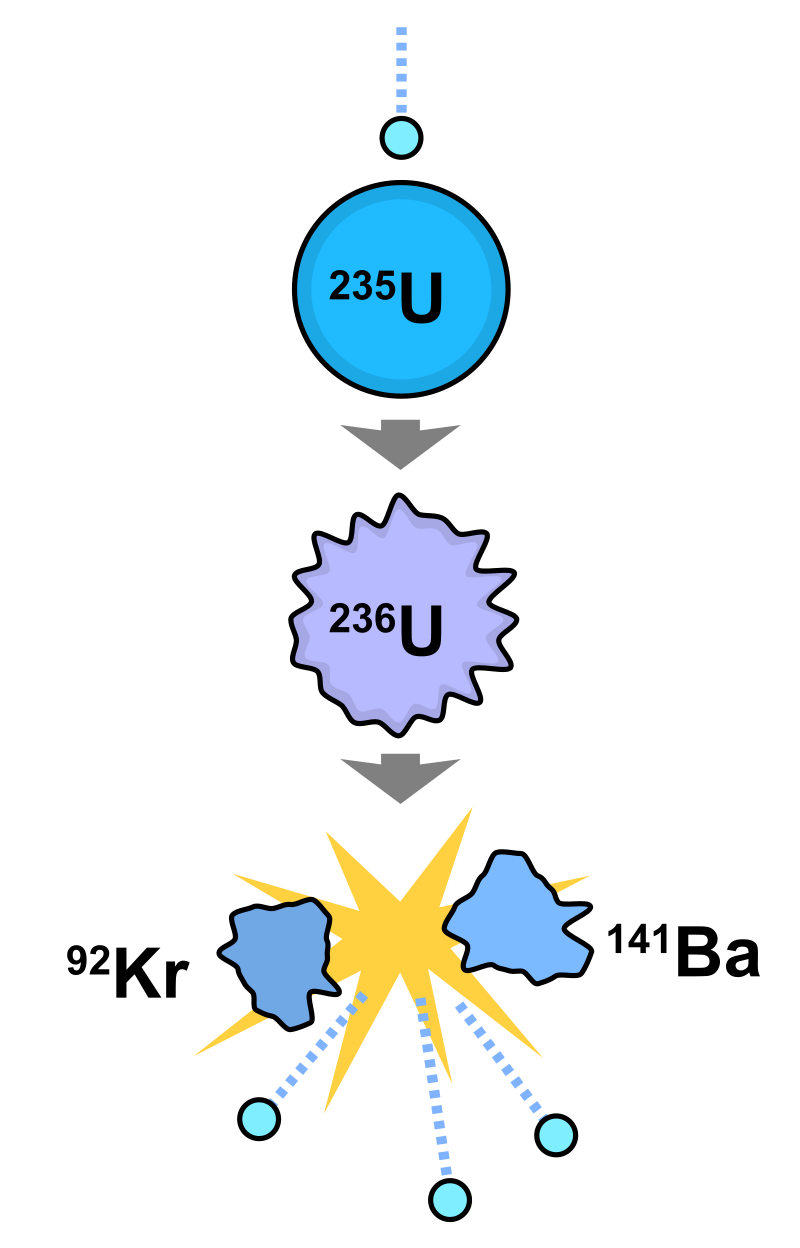
\includegraphics[width=0.4\textwidth]{../images/fission.png}
        \caption{Fission för uranium 235\parencite{figur1}}
        \label{fig:fission}
    \end{figure}

Det radioaktiva sönderfallet skapar också extremt mycket värme vilket betyder att reaktorn måste bli nerkyld.
Detta händer oftast med vatten.
Vattnet leder bort värmen som sedan omvandlar vattnet till ånga som driver en ångturbin.
\parencite{Nuclear_reactor}

    \begin{figure}
        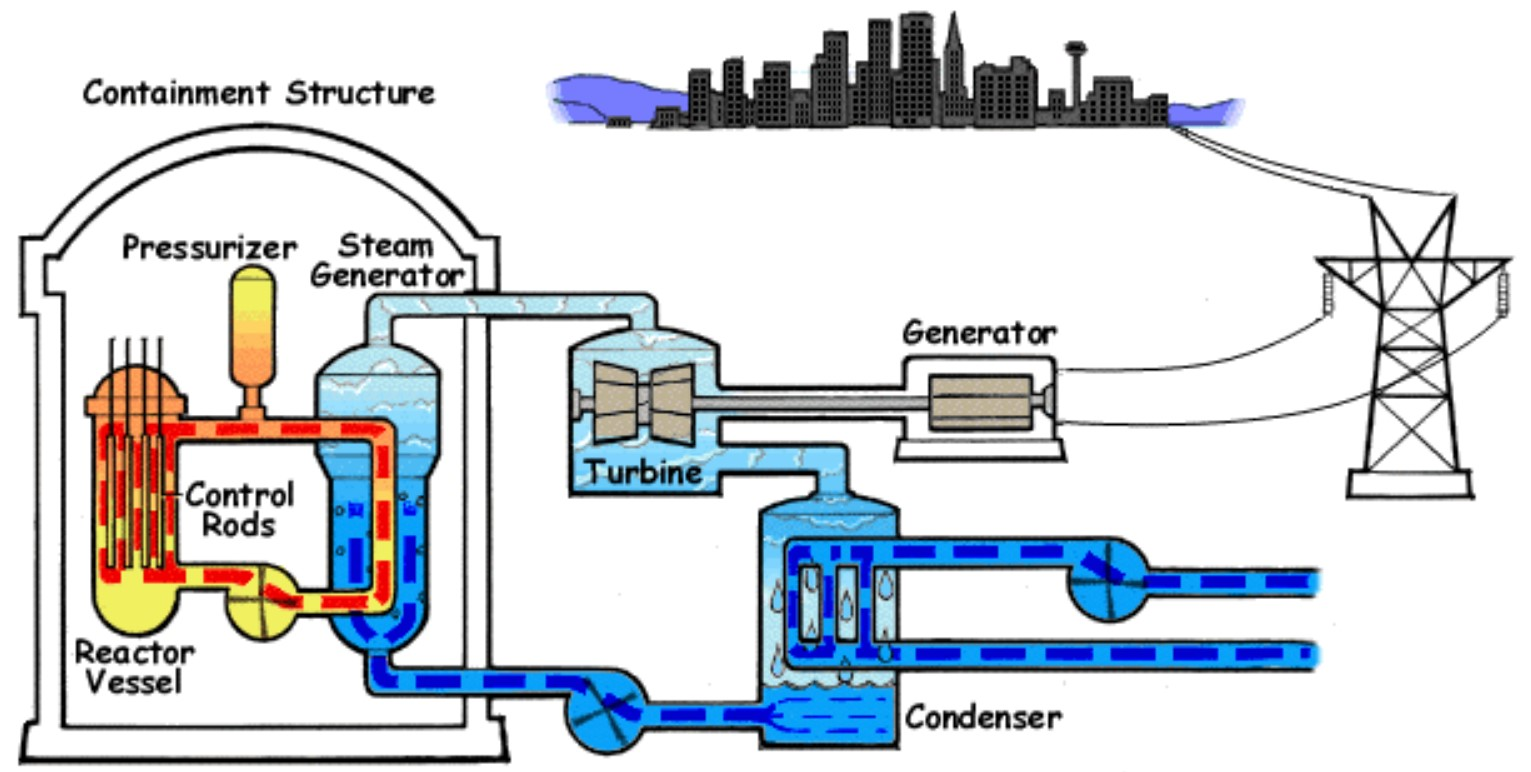
\includegraphics[width=0.8\textwidth]{../images/powerplant.jpg}
        \caption{Exempel på en kärnreaktor\parencite{figur2}}
        \label{fig:powerplant}
    \end{figure}
\newpage
    \subsection{Detta händer med radioaktivt avfall}\
Idag så börjar man med att låta det använda kärnbränslet förvaras i en vattenbassäng under ett år.
    I vattenbassängen kyls det använda kärnbränslet ner medans vattnet absorberar all strålning.
    Sedan transporteras det radioaktiva avfallet till en annan vattenbassäng som inte nödvändigtvis är brevid reaktorn.
    Där förvaras avfallet i ungefär 40 år.
    Slutligen så gjuts avfallet in i en behållare som består av en blandnig utav plåt, betong, cement och bitumen.
    Behållaren transporteras därefter till slutförvaring.\parencite{storage}
    Ungefär 96\% av radioaktivt avfall kommer inte till slutförvaring eftersom det deklareras som säkert och kan bli återvunnet.\parencite{recycle}

    \subsection{Miljö konsekvenser av uraniumgruvor}
    Uranium grävs oftast efter med dagbrottsbrytning eller normala gruvor.
    När gruvarbetet är klart så lämnas bara platsen.
    Detta betyder att resterna som är kvar tas inte hand om.
    Dam som kan innehålla en massa olika metaller inklusive radioaktiva ämnen sprids med vinden och vatten.
    Träd och andra växter som är i närheten kommer innehålla giftiga metaller.
    En del av det radioaktiva matrealet som är kvar sönderfaller till radon vilket kommer produceras i flera hundra år.\parencite{mining}

    \section{Slutsatser}

    Att gräva efter uranium förstör den närligande naturen.
    I slutändan så finns det inte kvar så mycket radioaktivt avfall och det som finns kvar hanteras säker.

    \printbibliography

\end{document}
